\section{Design of the Delay and \gls{reverb} Effect}
In this section, the delay and the \gls{reverb} will be designed to fit intro a \gls{dsp}, which mean that a discreet block diagram is obtained and afterwords the equation to the implementation is made. All the equation will afterwords be simulated in MATLAB and then the assembly code is developed and implemented. 


\subsection{Obtaining the Differential Equation}
The Delay effect use one of the effect block in the \gls{reverb} effect and therefore they will be presented and designed in the same section. The block diagram presented in \autoref{sec:reverberation} \autoref{fig:reverb_block} is changed so it fit intro a direct form 2 construction. 
The delay and \gls{reverb} effect both have \gls{iir} filter and \gls{fir} filter, but it is only the \gls{iir} filter which make the echo, the \gls{fir} filter is only applied to make a flat frequency respond in er delay effect and the two all pass filter in the \gls{reverb} effect, the seven first \gls{fir} filter is explained later. To get a naturally \gls{reverb} effect with the identical respond as a room acoustic respond and avoiding fluttering, all the serial \gls{reverb} unit needs to be an all pass filter and all parallel \gls{reverb} unit needs to be an \gls{lpcf} \citep{LPCF}. The\gls{lpcf} is used because the room acoustic characteristics is acting as a low pass filter, all low frequency signal will stay longer in the room than the high frequency \citep{rfi}. The \gls{reverb} needs to have at least 1000 echo per second, and the best way to make the \gls{reverb} effect is with four or six \gls{iir} filters in parallel and two all pass filter afterwords in serial, otherwise if there was not two all pass filter afterwords, it will require forty \gls{lpcf} to make 1000 echo per second \citep{natural_sounding_revorb}. The block diagram \autoref{fig:reverb_block_des} is in direct form 2 to minimize the implementation program. The delay and some of the \gls{reverb} effect can be obtained and is shown in \autoref{fig:reverb_block_des}. The \gls{reverb} effect is the one in red and black while the delay is only in red. 

\newpage

\begin{figure} [htbp]
 \centering
\begin{picture}(0,0)%
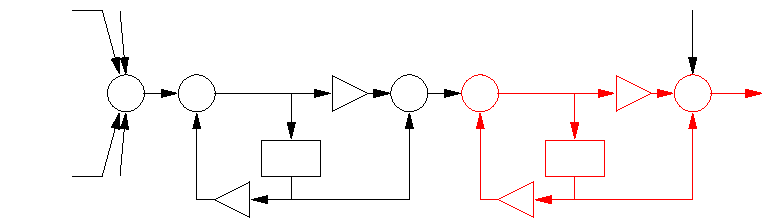
\includegraphics{reverb_diag_des.pdf}%
\end{picture}%
\setlength{\unitlength}{4144sp}%
%
\begingroup\makeatletter\ifx\SetFigFont\undefined%
\gdef\SetFigFont#1#2#3#4#5{%
  \reset@font\fontsize{#1}{#2pt}%
  \fontfamily{#3}\fontseries{#4}\fontshape{#5}%
  \selectfont}%
\fi\endgroup%
\begin{picture}(5832,1599)(-1319,-1288)
\put(3601,209){$x[n]$}%
\put(2656,-106){\color[rgb]{1,0,0}$w_8[n]$}%
\put(1711,-421){$\Sigma$}%
\put(721,-916){$z^{-d_7}$}%
\put( 91,-421){$\Sigma$}%
\put(1261,-196){$-\alpha$}%
\put(2251,-421){\color[rgb]{1,0,0}$\Sigma$}%
\put(2881,-916){\color[rgb]{1,0,0}$z^{-d_8}$}%
\put(271,-1006){$\alpha$}%
\put(2431,-1006){\color[rgb]{1,0,0}$\alpha$}%
\put(3871,-421){\color[rgb]{1,0,0}$\Sigma$}%
\put(3421,-196){\color[rgb]{1,0,0}$-\alpha$}%
\put(-449,-421){$\Sigma$}%
\put(-224,-106){$x_7[n]$}%
\put(1936,-106){\color[rgb]{1,0,0}$x_8[n]$}%
\put(4276,-106){\color[rgb]{1,0,0}$y[n]$}%
\put(-1304,-151){LPCF}%
\put(-1304,-421){filter in}%
\put(-1304,-646){Parallel}%
\end{picture}%

  \caption{The figure shows some of a block diagram of a \gls{reverb} and delay unit.}
  \label{fig:reverb_block_des}
\end{figure}

From \autoref{fig:reverb_block_des}, the following differential equations can be inferred for the delay effect, where the number 8 is omitted since the delay effect only is the the red all pass filter.

\begin{subequations}
\begin{equation}\label{eq:delay_eq}
       y[n] = - \alpha \cdot w[n] + w[n-d]
    \end{equation}
\begin{equation}\label{eq:delay_eq_in}
       w[n] = \alpha \cdot w[n-d] + x[n] 
    \end{equation}
 \end{subequations}
		
		

The \gls{reverb} unit is more advanced than the delay unit and before the differential equations can be inferred, some calculation is needed. The \gls{reverb} unit calculation are based on an article \citep{natural_sounding_revorb} which explain the design parametric for a Schroeder \gls{reverb} processor unit very well. Form \citep{natural_sounding_revorb} the \gls{reverb} time is defined by \autoref{eq:reverb_defined}



\begin{equation}
\label{eq:reverb_defined}
		T = \frac{60}{-20 \cdot log(\alpha)} \cdot \tau
\end{equation}

    \startexplain
\explain{$60$ is the \gls{reverb} attenuation in \si{\decibel}, and the \gls{reverb} time is defined that a given signal is attenuated by \SI{60}{\decibel}}{\si{\decibel}}
\explain{$\tau$ is the delay time}{\si{\second}}
\explain{$T$ is the resulting \gls{reverb} time}{\si{\second}}
\explain{$-20 \cdot log10(\alpha)$ is the attenuation in the feedback loop for each round}{\si{\decibel}}
    \stopexplain

Both the positive and negative gain $\alpha$ is defined to be ether 0.708  \citep{natural_sounding_revorb} and the total \gls{reverb} echo density shall at lest be 1000 echo per second. In formula \autoref{eq:reverb_defined_tal_res} it can be obtain that $\tau$ shall be $\frac{1}{20}$ with a $T$ of one second.


\begin{subequations}
\begin{equation}\label{eq:reverb_defined_tal}
       T = \frac{60}{-20 \cdot log10(0.708)} \cdot \tau
       \addunit{\si{\second}}
    \end{equation}
\centering
$\Updownarrow$
\begin{equation}\label{eq:reverb_defined_tal_res}
        \tau = \frac{1}{20} T
        \addunit{\si{\second}}
    \end{equation}
 \end{subequations}

\autoref{eq:reverb_defined_tal_res} then shows that the $\tau$ time is \SI{50}{\milli\second} with a total \gls{reverb} time $T$ of \SI{1}{second}. This achieve an echo density of 20 echo per second for each of the \gls{lpcf} filter, but if all the filter have the same delay time some echo will interference. To avoid interference each filter delay time is chosen to its own prime numbers which lay beneath \SI{50}{\milli\second} The chosen delay prime number is as following \autoref{tab:reverb_delay}, and there are chosen six, so it is possible to design a Moorer \gls{reverb} unit \citep{DAFX}. The same applies in the chose of \autoref{tab:reverb_bgain}.

\begin{table}[htbp]
\centering
\caption{The chosen delay prime numbers}
\label{tab:reverb_delay}
\begin{tabular}{lll}
$d_1$ & = & 19 \\ 
$d_2$ & = & 23 \\ 
$d_3$ & = & 29 \\ 
$d_4$ & = & 31 \\ 
$d_5$ & = & 37 \\
$d_6$ & = & 41 \\
$d_7$ & = & 17 \\
$d_8$ & = & 13
\end{tabular}
\end{table}

Each \gls{lpcf} filter is also attenuated by a defined gain which is shown in \autoref{tab:reverb_bgain}

\begin{table}[htbp]
\centering
\caption{The chosen delay prime numbers}
\label{tab:reverb_bgain}
\begin{tabular}{lll}
$b_1$ & = & 1 \\
$b_2$ & = & 0.9 \\
$b_3$ & = & 0.8 \\
$b_4$ & = & 0.7 \\
$b_5$ & = & 0.6 \\
$b_6$ & = & 0.5 
\end{tabular}
\end{table}


The \gls{reverb} unit require 1000 echo per second \citep{natural_sounding_revorb}. To achieve natural \gls{reverb} sound there needs to be multiply all pass filter delay unit in serial after the six \gls{lpcf} in parallel. It is defined by \citep{natural_sounding_revorb} that two all pass filter is required to make a natural \gls{reverb} sound.
To calculate the approximated number of echo in one second from six \gls{lpcf}, the following is consiteret. The total numbers of echo over \SI{-60}{\decibel} is added together form each \gls{iir} filter together because each \gls{lpcf} have its own prime number. The result is 120 echo per second because each \gls{lpcf} make 20 echo. The following calculation \autoref{eq:reverb_ser} calculate the approximate resulting echo after the first all pass filter if non of the echo interference and the attenuation form \autoref{tab:reverb_bgain} is included. Both the first and the second all pass have a prime number under 50, so each signal from the all pass filter will be repeated maximum of $24$ times before the signal is attenuated under \SI{60}{\decibel}.


\begin{subequations}
\begin{equation}\label{eq:reverb_ser}
      \text{aprox  echo} = \sum_{x=0}^{19} 20-x + \sum_{x=0}^{17} 18-x + \sum_{x=0}^{15} 16-x + \sum_{x=0}^{13} 14-x+ \sum_{x=0}^{11} 12-x+ \sum_{x=0}^{9} 10-x
    \end{equation}
\centering
$\Updownarrow$
\begin{equation}\label{eq:reverb_seriel}
        \text{aprox echo from first all pass filter} = 755
        \addunit{\si{1}}
    \end{equation}
 \end{subequations}

    \startexplain
\explain{$20$ echo is calculated from each echo from the second \gls{iir} filter which is attenuated 10 percent, $echo=\left \lfloor 20 \cdot b_2 \right \rfloor$ }{\si{1}}
\explain{$18$ echo is calculated from each echo from the third \gls{iir} filter which is attenuated 20 percent, $echo=\left \lfloor 20 \cdot b_3 \right \rfloor$ }{\si{1}}
\explain{$16$ echo is calculated from each echo from the fourth \gls{iir} filter which is attenuated 30 percent, $echo=\left \lfloor 20 \cdot b_4 \right \rfloor$ }{\si{1}}
\explain{$16$ echo is calculated from each echo from the fourth \gls{iir} filter which is attenuated 40 percent, $echo=\left \lfloor 20 \cdot b_4 \right \rfloor$ }{\si{1}}
\explain{$16$ echo is calculated from each echo from the fourth \gls{iir} filter which is attenuated 50 percent, $echo=\left \lfloor 20 \cdot b_4 \right \rfloor$ }{\si{1}}
    \stopexplain

Since the echo density already is about 1038 echo per second, the last \gls{fir} filter will defenetly have a echo density of over 1000 echo per second for the output of the \gls{reverb} effect. In \citep{DAFX} Moorer suggests adding two extra \gls{iir} filter in parallel an making an early reflection network. The early reflection network is a simple multi tap \gls{fir} filter constellation. Moorer also suggests to inset a low pass filter in the feedback for the \gls{iir} filters, where the room is scaled by changing the feedback gain. The following formula \autoref{eq:reverb_eq_eks} shows the formula of the low pass feedback comb filter \citep{LPCFfd}. 

\begin{subequations}\label{eq:reverb_eq_eks}
    \begin{equation}\label{eq:reverb_eq_iireks1}
    w_1[n] = x_1[n] + L_D \cdot w_1[n-1] + f \cdot (1-L_D) \cdot x_2[n-d_1]
    \end{equation}
\begin{equation}\label{eq:reverb_eq_iireks2}
x_2[n] = w_1[n] - L_D \cdot w_1[n-1]
    \end{equation}
 \end{subequations}

Where:\\ \\

The $f$ is defining the room size, and the equation of $f$ is as following \autoref{eq:reverb_eq_f} where scaleroom is used to scale the room size \citep{LPCFfd}.

\begin{subequations}\label{eq:reverb_eq_f}
\begin{equation}\label{eq:reverb_eq_f1}
    f = \text{roomsize} = \text{initialroom} \cdot \text{scaleroom} + \text{offsetroom}
    \end{equation}
\centering
$\Updownarrow$
\begin{equation}\label{eq:reverb_eq_f1}
    f = 0.5 \cdot \text{scaleoom} + 0.7
    \end{equation}
 \end{subequations}   
   
The $L_D$ is defining the room damping, and the equation of $L_D$ is as following \autoref{eq:reverb_eq_L_D} where scaledamp is used to scale the room damping \citep{LPCFfd}.    

\begin{subequations}\label{eq:reverb_eq_L_D}
\begin{equation}\label{eq:reverb_eq_L_D1}
    L_D = \text{damp} = \text{initialdamp} \cdot \text{scaledamp}
    \end{equation}
\centering
$\Updownarrow$
\begin{equation}\label{eq:reverb_eq_L_D1}
    L_D = 0.5 \cdot \text{scaledamp}
    \end{equation}
 \end{subequations}   


   The following \autoref{fig:reverb_block_design} shows a direct form 2 block diagram over the \gls{reverb} unit.


\begin{figure} [htbp]
 \centering
\begin{picture}(0,0)%
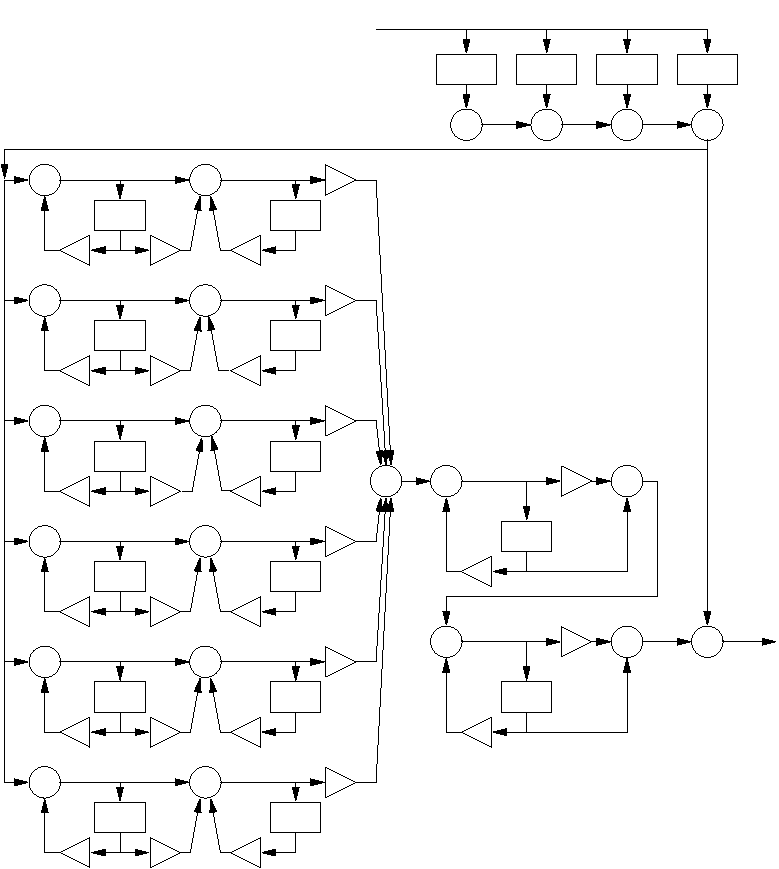
\includegraphics{reverb_serial_des.pdf}%
\end{picture}%
\setlength{\unitlength}{3646sp}%
%
\begingroup\makeatletter\ifx\SetFigFont\undefined%
\gdef\SetFigFont#1#2#3#4#5{%
  \reset@font\fontsize{#1}{#2pt}%
  \fontfamily{#3}\fontseries{#4}\fontshape{#5}%
  \selectfont}%
\fi\endgroup%
\begin{picture}(6819,12186)(-3656,-5608)
\put(-3194,-511){$f$}%
\put(1711,-421){$\Sigma$}%
\put(721,-916){$z^{-d_7}$}%
\put( 91,-421){$\Sigma$}%
\put(1261,-196){$-\alpha$}%
\put(271,-1006){$\alpha$}%
\put(-449,-421){$\Sigma$}%
\put(-224,-106){$x_7[n]$}%
\put(1936,-106){$x_8[n]$}%
\put( 91,-1861){$\Sigma$}%
\put(1711,-1861){$\Sigma$}%
\put(271,-2446){$\alpha$}%
\put(721,-2356){$z^{-d_8}$}%
\put(1261,-1636){$-\alpha$}%
\put(2701,-1636){$y[n]$}%
\put(2431,-1861){$\Sigma$}%
\put(-764,4934){$x_1[n]$}%
\put(-2204,-3571){$-L_D$}%
\put(-2339,-2941){$w_5[n]$}%
\put(-2789,-3436){$z^{-1}$}%
\put(-3239,-3571){$L_D$}%
\put(-1484,-2941){$x_6[n]$}%
\put(-3374,-3121){$\Sigma$}%
\put(-1754,-3121){$\Sigma$}%
\put(-764,-2941){$b_5$}%
\put(-2789,-2806){$z^{-d_5}$}%
\put(-3194,-2311){$f$}%
\put(-2789,-5236){$z^{-1}$}%
\put(-3239,-5371){$L_D$}%
\put(-2204,-5371){$-L_D$}%
\put(-3374,-4921){$\Sigma$}%
\put(-1484,-4741){$x_7[n]$}%
\put(-2339,-4741){$w_6[n]$}%
\put(-2789,-4606){$z^{-d_6}$}%
\put(-3194,-4111){$f$}%
\put(-1754,-4921){$\Sigma$}%
\put(-764,-4741){$b_6$}%
\put(-2789,-1636){$z^{-1}$}%
\put(-3374,-1321){$\Sigma$}%
\put(-2204,-1771){$-L_D$}%
\put(-3239,-1771){$L_D$}%
\put(-1754,-1321){$\Sigma$}%
\put(-2339,-1141){$w_4[n]$}%
\put(-2789,-1006){$z^{-d_4}$}%
\put(-1484,-1141){$x_5[n]$}%
\put(-764,-1141){$b_4$}%
\put(-3374,479){$\Sigma$}%
\put(-2789,164){$z^{-1}$}%
\put(-3239, 29){$L_D$}%
\put(-1484,659){$x_4[n]$}%
\put(-2204, 29){$-L_D$}%
\put(-1754,479){$\Sigma$}%
\put(-2789,794){$z^{-d_3}$}%
\put(-2339,659){$w_3[n]$}%
\put(-3194,1289){$f$}%
\put(-764,659){$b_3$}%
\put(-3374,2279){$\Sigma$}%
\put(-3239,1829){$L_D$}%
\put(-2789,1964){$z^{-1}$}%
\put(-2204,1829){$-L_D$}%
\put(-2789,2594){$z^{-d_2}$}%
\put(-1754,2279){$\Sigma$}%
\put(-764,2459){$b_2$}%
\put(-1484,2459){$x_3[n]$}%
\put(-2339,2459){$w_2[n]$}%
\put(-3284,3089){$f$}%
\put(-1754,4079){$\Sigma$}%
\put(-3374,4079){$\Sigma$}%
\put(-2789,4394){$z^{-d_1}$}%
\put(-2789,3764){$z^{-1}$}%
\put(-764,4259){$b_1$}%
\put(-1484,4259){$x_2[n]$}%
\put(-2339,4259){$w_1[n]$}%
\put(-3239,3629){$L_D$}%
\put(-2204,3629){$-L_D$}%
\put(-3284,4889){$f$}%
\put(-3464,6419){$x[n]$}%
\put(-1439,5879){$z^{-ed_3}$}%
\put(-719,5879){$z^{-ed_4}$}%
\put(-2744,5384){$\Sigma$}%
\put(-2024,5384){$\Sigma$}%
\put(-1304,5384){$\Sigma$}%
\put(-2159,5879){$z^{-ed_2}$}%
\put(-2879,5879){$z^{-ed_1}$}%
\put(-584,5384){$\Sigma$}%
\end{picture}%
  \caption{The figure shows a block diagram of a \gls{reverb} unit.}
  \label{fig:reverb_block_design}
\end{figure}

\newpage
The equation for the \gls{reverb} can be written in 18 parts as following \autoref{eq:reverb_eq}


\begin{subequations}\label{eq:reverb_eq}
\begin{equation}\label{eq:reverb_eq_ed}
		x_1[n] = x[n]+x[n-ed_1]+x[n-ed_2]+x[n-ed_3]+x[n-ed_4]
    \end{equation}
    
\begin{equation}\label{eq:reverb_eq_iir1w}
    w_1[n] = x_1[n] + L_D \cdot w_1[n-1] + f \cdot (1-L_D) \cdot x_2[n-d_1]
    \end{equation}
\begin{equation}\label{eq:reverb_eq_iir1x}
x_2[n] = w_1[n] - L_D \cdot w_1[n-1]
    \end{equation}
    
\begin{equation}\label{eq:reverb_eq_iir2w}
    w_2[n] = x_1[n] + L_D \cdot w_2[n-1] + f \cdot (1-L_D) \cdot x_3[n-d_1]
    \end{equation}
\begin{equation}\label{eq:reverb_eq_iir2x}
x_3[n] = w_2[n] - L_D \cdot w_2[n-1]
    \end{equation}
    
\begin{equation}\label{eq:reverb_eq_iir3w}
    w_3[n] = x_1[n] + L_D \cdot w_3[n-1] + f \cdot (1-L_D) \cdot x_4[n-d_1]
    \end{equation}
\begin{equation}\label{eq:reverb_eq_iir3x}
x_4[n] = w_3[n] - L_D \cdot w_3[n-1]
    \end{equation}
    
\begin{equation}\label{eq:reverb_eq_iir4w}
    w_4[n] = x_1[n] + L_D \cdot w_4[n-1] + f \cdot (1-L_D) \cdot x_5[n-d_1]
    \end{equation}
\begin{equation}\label{eq:reverb_eq_iir4x}
x_5[n] = w_4[n] - L_D \cdot w_4[n-1]
    \end{equation}
    
\begin{equation}\label{eq:reverb_eq_iir5w}
    w_5[n] = x_1[n] + L_D \cdot w_5[n-1] + f \cdot (1-L_D) \cdot x_6[n-d_1]
    \end{equation}
\begin{equation}\label{eq:reverb_eq_iir5x}
x_6[n] = w_5[n] - L_D \cdot w_5[n-1]
    \end{equation}
    
\begin{equation}\label{eq:reverb_eq_iir6w}
    w_6[n] = x_1[n] + L_D \cdot w_6[n-1] + f \cdot (1-L_D) \cdot x_7[n-d_1]
    \end{equation}
\begin{equation}\label{eq:reverb_eq_iir6x}
x_7[n] = w_6[n] - L_D \cdot w_6[n-1]
    \end{equation}
    
\begin{equation}\label{eq:reverb_eq_iirto}
    \begin{array}[b]{r}
      x_8[n] = x_2[n] \cdot b_1+x_3n] \cdot b_2+x_4[n] \cdot b_3\\
+x_5[n] \cdot b_4+x_6[n] \cdot b_5+x_7[n] \cdot b_6
    \end{array}
    \end{equation}
    
    \begin{equation}\label{eq:reverb_eq_ap1}
w_8[n] = \alpha_7 \cdot w[n-d_8] + x_8[n] 
    \end{equation}
\begin{equation}\label{eq:reverb_eq_ap12}
x_9[n] = - \alpha_8 \cdot w_8[n] + w_8[n-d_7]
    \end{equation}
    
    \begin{equation}\label{eq:reverb_eq_ap2}
w_9[n] = \alpha_8 \cdot w[n-d_8] + x_9[n] 
    \end{equation}
    \begin{equation}\label{eq:reverb_eq_ap22}
y[n] = - \alpha_8 \cdot w_9[n] + w_9[n-d_8] + x_1[n]
    \end{equation}
\end{subequations}


\subsection{Matlab Simulation}

A delay can be done in different ways digitally. One way is to use a ring buffer also known as circular buffer. \\
The idea of this data structure is that it takes values and only outputs them when it gets full, and overwrites the oldest after outputting it. It is a kind of a FIFO queue structure but where the start and the overwriting can start at any index. \\
This means that the size of the buffer depends on the delay.  The buffer size must then be always up-to-date with the new delay value. \\ 

The Matlab code for the delay effect is as following \autoref{code:delay_sim}

\includeCode{delay.m}{matlab}{1}{39}{The delay simulation matlab code}{code:close}{code/design/}\label{code:delay_sim}


Applying one sinus round gives the following result

\begin{figure}[htbp]
	\centering
	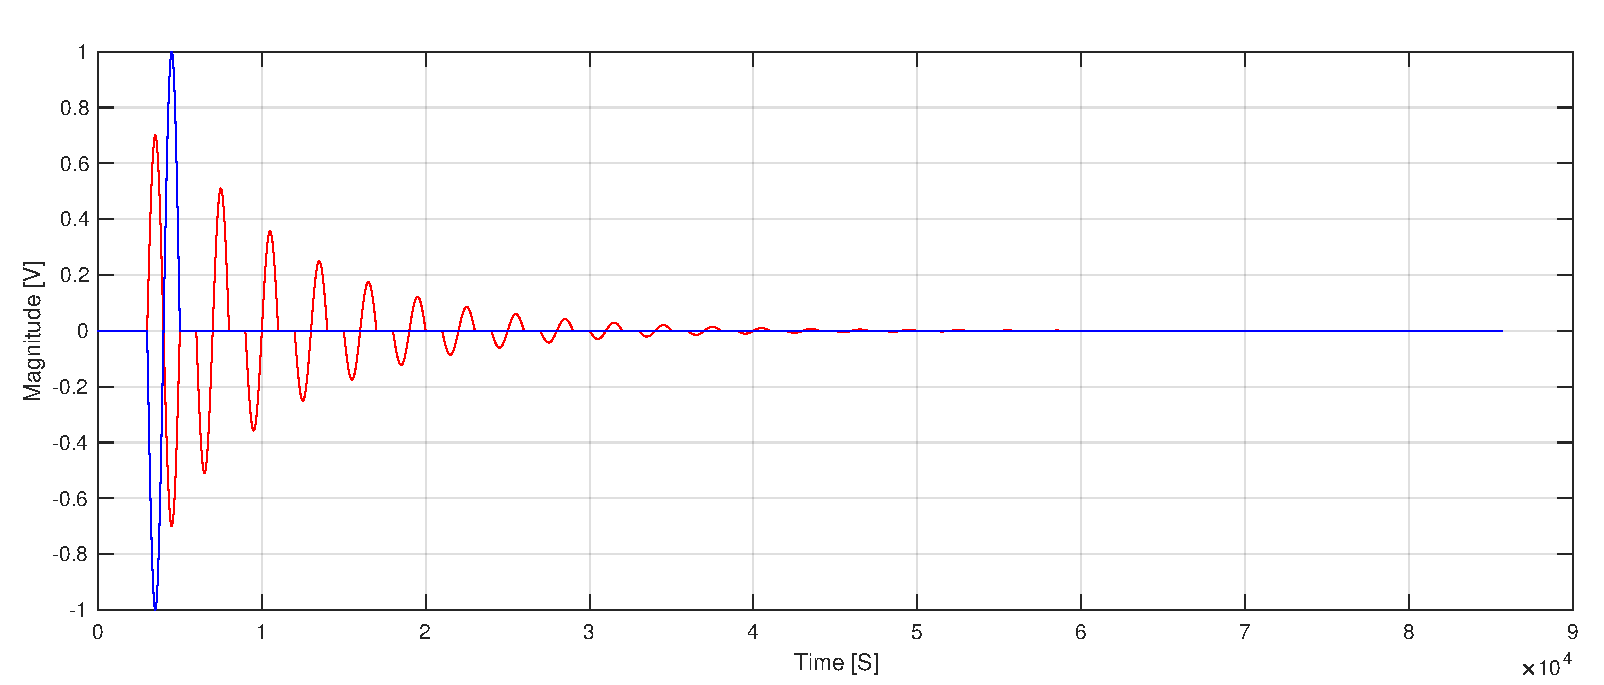
\includegraphics[width=1\textwidth]{delay}
	\caption{The plot shows the result for the \autoref{code:delay}}
	\label{fig:delay_plot}
\end{figure}



\begin{figure}[htbp]
	\centering
	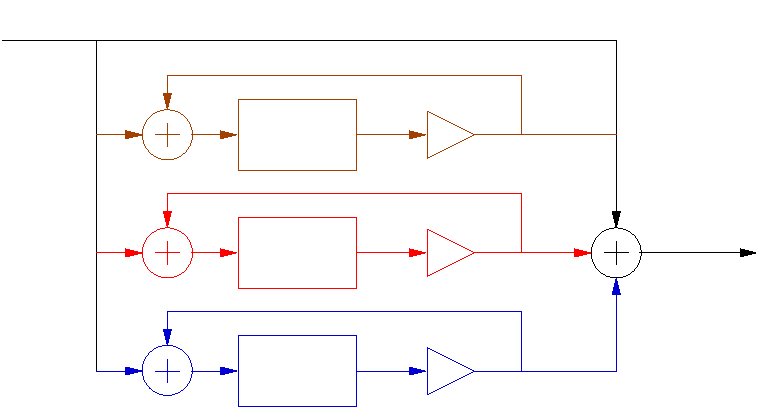
\includegraphics[width=0.8\textwidth]{reverb}
	\caption{The plot shows the result for the \autoref{code:delay}}
	\label{fig:delay_plot}
\end{figure}